\documentclass{article}

\usepackage{graphicx}
\usepackage{tikz}
\usepackage{tikzsymbols}
\usetikzlibrary{calc,patterns,shapes.geometric}
\pagestyle{empty}
\usepackage[margin=0pt]{geometry}
\geometry{papersize={14in,12in}}

\def\centerarc[#1](#2)(#3:#4:#5){\draw[#1] ($(#2)+({#5*cos(#3)},{#5*sin(#3)})$) arc (#3:#4:#5);}

\begin{document}
	\begin{figure}
		\centering
		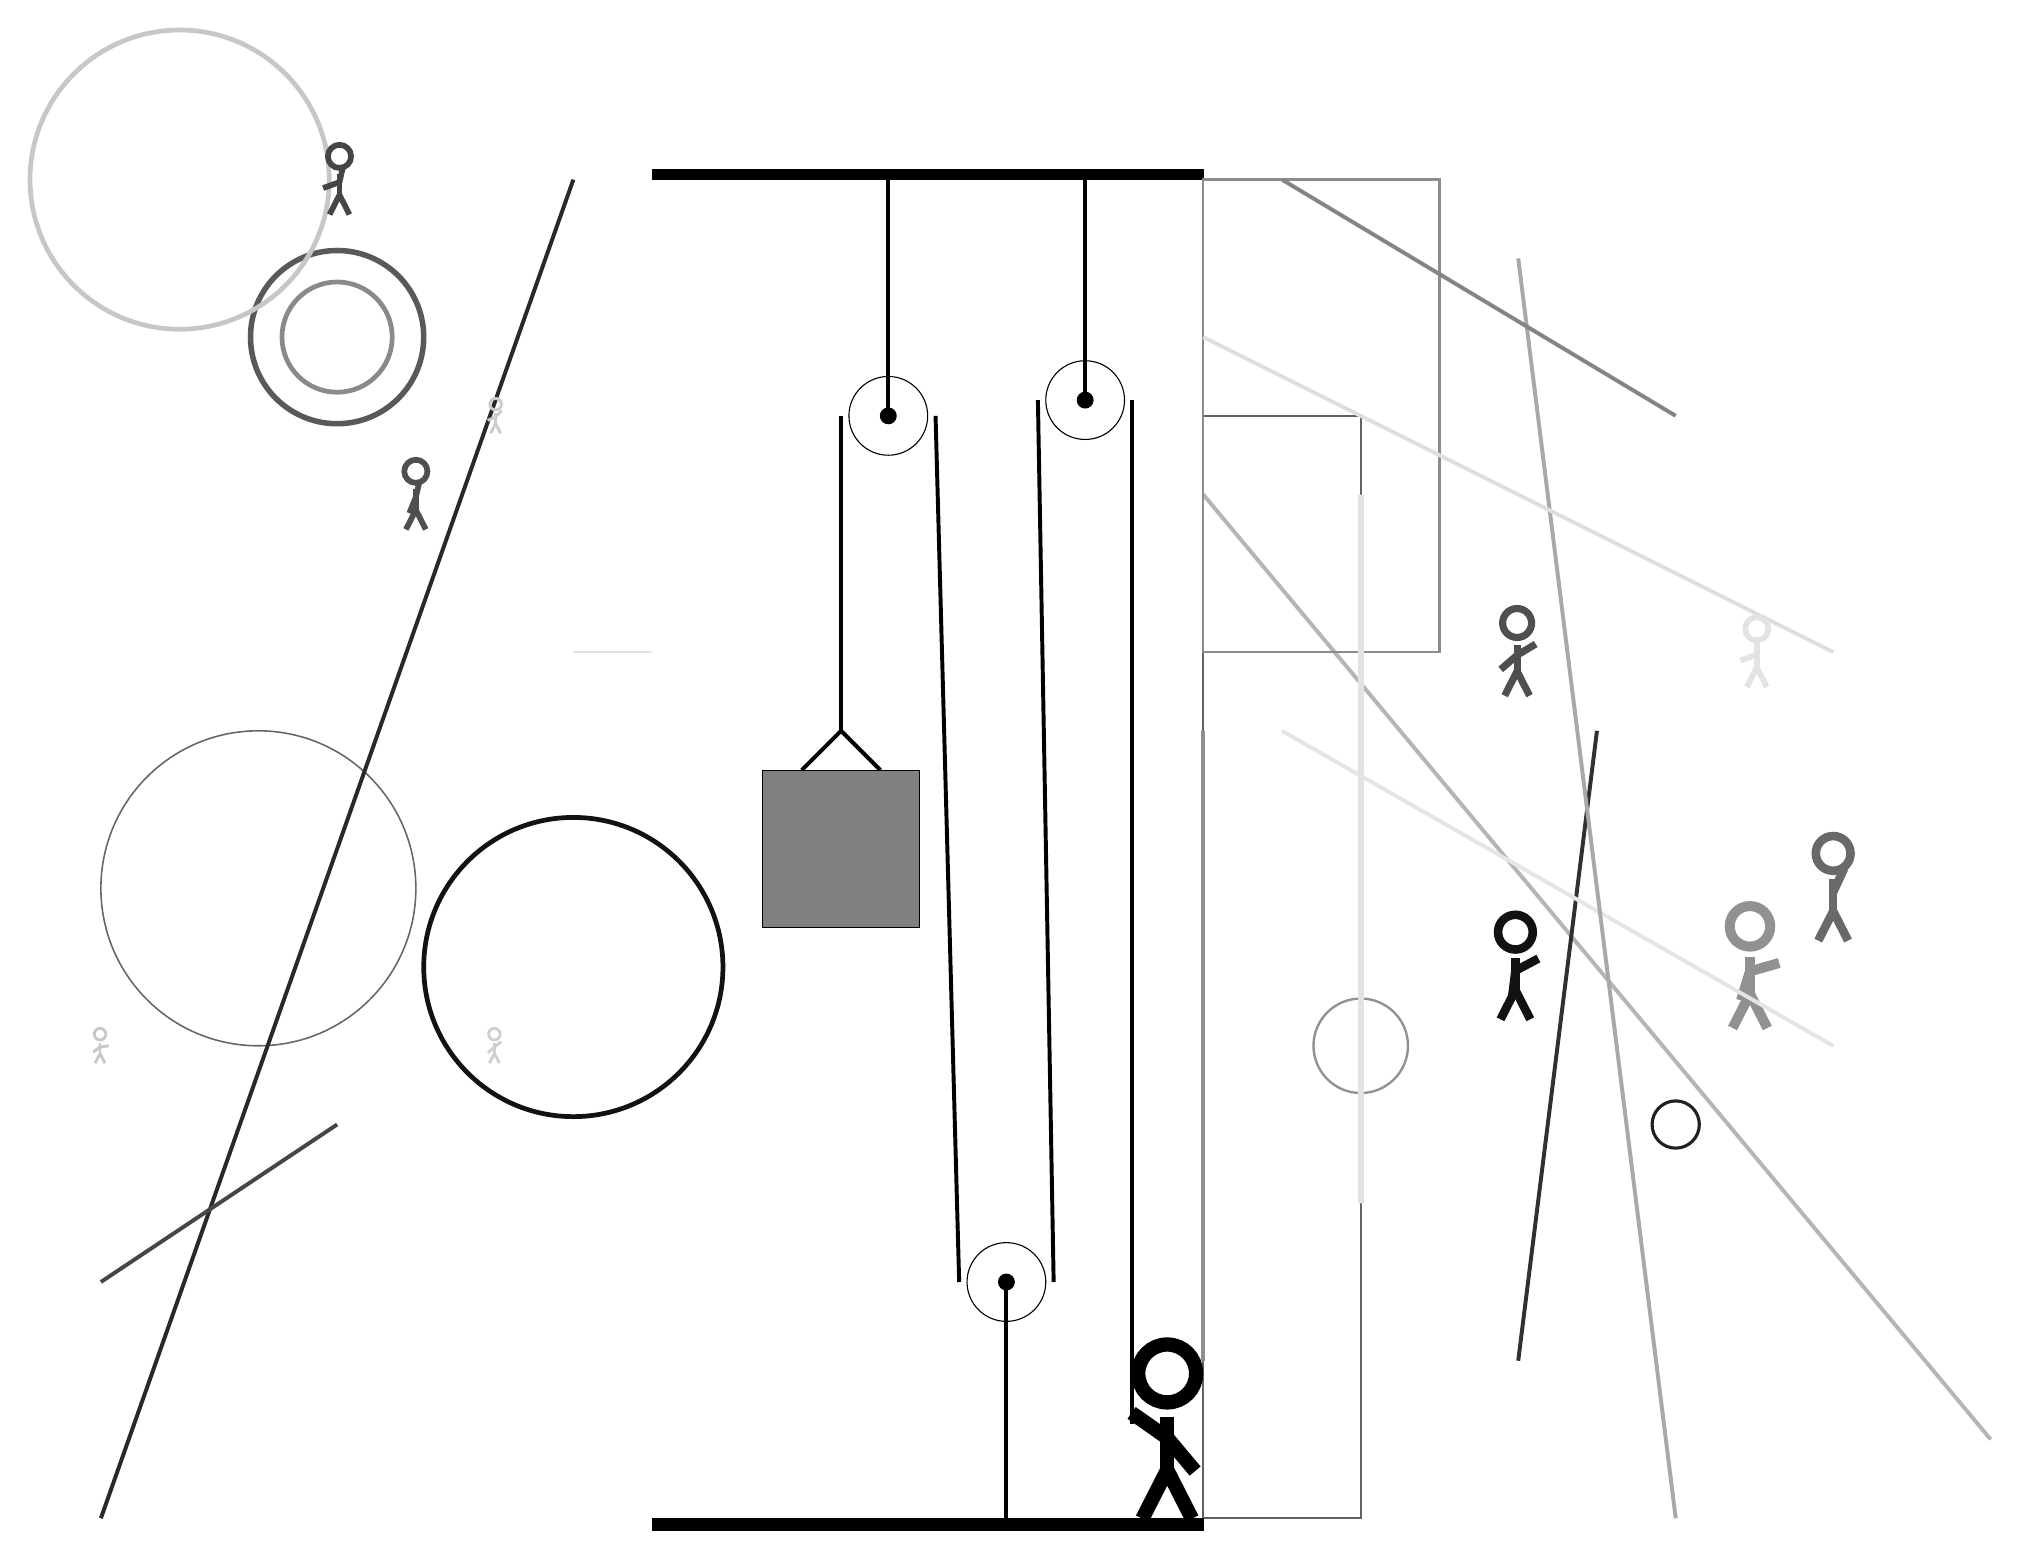
\begin{tikzpicture}
			%%%%% START %%%%%
			
			\draw[fill=black] (-2, 14) rectangle (5, 14.125);
			
			\draw (1, 11) circle (0.5);
			\draw[fill=black] (1, 11) circle (0.1);
			\draw[line width=0.5mm]  (1, 14) -- (1, 11);
			
			\draw[fill=white](2.5, 0) circle (0.5);
			\draw[fill=black] (2.5, 0) circle (0.1);
			\draw[line width=0.5mm]  (2.5, -3) -- (2.5, 0);
			
			\draw[line width=0.2mm, color=black!63] (5, -3) rectangle (5, -3);
			
			\draw [line width=0.2mm, color=black!60](-7, 5) circle (2.0);
			\draw [line width=0.7mm, color=black!65](-6, 12) circle (1.1);
			\draw[line width=0.5mm, color=black!84](-3, 14) -- (-9, -3);
			
			\draw[line width=0.2mm, color=black!11] (-3, 8) rectangle (-2, 8);
			\node[line width=0.2mm, color=black!69] at (9, 8) {\Strichmaxerl[5][41][31]};
			
			\draw [line width=0.4mm, color=black!87](11, 2) circle (0.3);
			
			\node[line width=0.6mm, color=black!43] at (12, 4) {\Strichmaxerl[7][73][16]};
			\draw [line width=0.6mm, color=black!22](-8, 14) circle (1.9);
			\node[line width=0.7mm, color=black!59] at (13, 5) {\Strichmaxerl[6][90][65]};
			\node[line width=0.5mm, color=black!19] at (-4, 3) {\Strichmaxerl[2][42][38]};
			
			\draw[line width=0.5mm, color=black!29](5, 10) -- (15, -2);
			\draw[line width=0.5mm, color=black!72](-6, 2) -- (-9, 0);
			\draw[line width=0.5mm, color=black!81](9, -1) -- (10, 7);
			\draw[line width=0.5mm, color=black!10](6, 7) -- (13, 3);
			\node[line width=0.2mm, color=black!93] at (9, 4) {\Strichmaxerl[6][83][28]};
			\draw[line width=0.5mm, color=black!34](9, 13) -- (11, -3);
			\draw[line width=0.2mm, color=black!61] (7, -3) rectangle (5, 11);
			\draw[line width=0.3mm, color=black!45] (5, 14) rectangle (8, 8);
			
			\draw[line width=0.5mm, color=black!48](6, 14) -- (11, 11);
			\draw[line width=0.5mm, color=black!13](5, 12) -- (13, 8);
			\draw [line width=0.3mm, color=black!43](7, 3) circle (0.6);
			
			\draw[line width=0.5mm, color=black!44](5, 7) -- (5, -1);
			\node[line width=0.6mm, color=black!22] at (-9, 3) {\Strichmaxerl[2][37][8]};
			\draw [line width=0.6mm, color=black!93](-3, 4) circle (1.9);
			
			\node[line width=0.5mm, color=black!11] at (12, 8) {\Strichmaxerl[4][20][90]};
			\node[line width=0.2mm, color=black!69] at (-5, 10) {\Strichmaxerl[4][68][77]};
			\node[line width=0.6mm, color=black!20] at (-4, 11) {\Strichmaxerl[2][22][47]};
			\node[line width=0.3mm, color=black!73] at (-6, 14) {\Strichmaxerl[4][20][77]};
			
			\draw[line width=0.7mm, color=black!11] (7, 10) rectangle (7, 1);
			\draw [line width=0.6mm, color=black!46](-6, 12) circle (0.7);
			
			
			\draw[fill=white](3.5, 11.2) circle (0.5);
			\draw[fill=black] (3.5, 11.2) circle (0.1);
			\draw[line width=0.5mm] (3.5, 14) -- (3.5, 11.2);
			
			\draw[line width=0.5mm] (-0.1, 6.5) -- (0.4, 7.0) -- (0.9, 6.5);
			\draw[fill=black!50] (-0.6, 6.5) rectangle (1.4, 4.5);
			
			\draw[line width=0.5mm] (0.4, 11) -- (0.4, 7.0);
			\centerarc[line width=0.5mm](1, 11)(0:180:0.6);
			\draw[line width=0.5mm](1.6, 11) -- (1.9, 0);
			\centerarc[line width=0.5mm](2.5, 0)(180:360:0.6);
			\draw[line width=0.5mm](3.1, 0) -- (2.9, 11.2);
			\centerarc[line width=0.5mm](3.5, 11.2)(0:180:0.6);
			\draw[line width=0.5mm](4.1, 11.2) -- (4.1, -1.8);
			
			\node at (4.5, -1.9) {\Strichmaxerl[10][-35][-50]};
			
			\draw[fill=black] (-2, -3) rectangle (5, -3.15);
			
			%%%%% END %%%%%
		\end{tikzpicture}
	\end{figure}	
\end{document}